\subtitle{Emisiones en rellenos sanitarios}
\begin{frame}
  \titlepage
\end{frame}

\section{Introducción}

\begin{frame}{}

	Los principales constituyentes de los gases generados en rellenos son \textbf{CH4}y \textbf{CO2}. 
	Se producen por microorganismos bajo condiciones anaerobicas.
	La produccion de gas sigue las siguientes fases:
        \begin{center}
            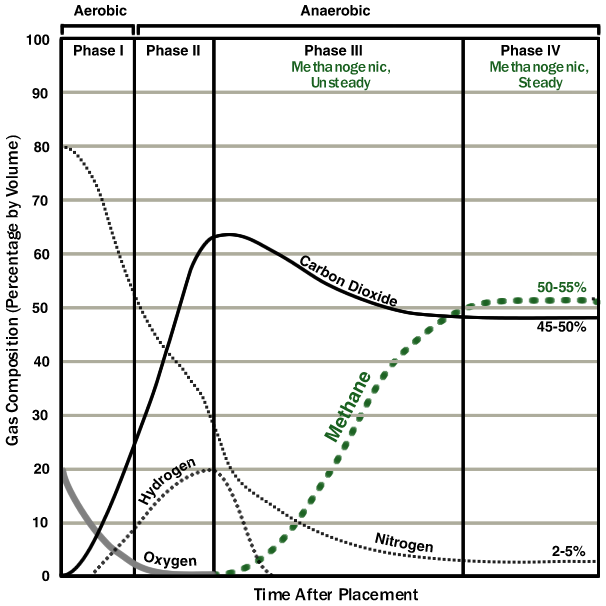
\includegraphics[width=0.6\textwidth]{img/landfillgas.png}
        \end{center}
	%\begin{itemize}
	%	\item Aerobica: oxidación de compuestos orgánicos complejos mediado por O2.
	%	\item Anaerobica: extincion de O2, generando condiciones anaerobicas, donde se produce mucho CO2, y H2.
	%	\item Anaerobica: comienza produccion de CH4, la produccion de CO2 empieza a decrecer,. El N2 se nde se produce mucho CO2, y H2.
	%\end{itemize}

\end{frame}
